
\documentclass{article}
\title{Labwork 6: CNN}
\author{Nguyen Dang Minh - M23.ICT.008}
\date{\today}

\usepackage{booktabs}
\usepackage{amsmath}
\begin{document}

\maketitle

\section{Introduction}
Convolutional Neural Networks (CNNs) are a class of deep learning algorithms that are particularly powerful for analyzing visual data. They are widely used in image and video recognition, medical image analysis, and other computer vision tasks.


\section{Architecture}
A typical CNN architecture consists of several types of layers:

\subsection{Convolutional Layer}
The convolutional layer is the core of a CNN. It consists of a set of learnable kernels that slide over the input data to produce feature maps.

\subsection{Activation Function}
After the convolution, an activation function is applied. The most commonly used activation function is ReLU, defined as:
\[
\text{ReLU}(x) = \max(0, x)
\]

\subsection{Pooling Layer}
Pooling layers reduce the dimensions of the feature maps to reduce complexity, which improve the training time and predict.

\subsection{Fully Connected Layer}
We processed in a traditional neural network for simple classfication for the number of unique classes that dataset has.

It works like labwork 5 custom neural network we have done.

\subsection{My architecture }
This is the structure of my data. I opted not to use VGG19 because my dataset is relatively small, and the results with VGG19 were not satisfactory. Instead, I use a smaller, custom CNN:


\begin{table}[h!]
    \centering
    \begin{tabular}{|l|c|c|}
    \hline
    \textbf{Layer (type)}         & \textbf{Output Shape} & \textbf{Param \#} \\ \hline
    conv2d (Conv2D)               & (None, 254, 254, 32)  & 896               \\ \hline
    max\_pooling2d (MaxPooling2D) & (None, 127, 127, 32)  & 0                 \\ \hline
    conv2d\_1 (Conv2D)            & (None, 125, 125, 64)  & 18,496            \\ \hline
    max\_pooling2d\_1 (MaxPooling2D) & (None, 62, 62, 64)  & 0                 \\ \hline
    conv2d\_2 (Conv2D)            & (None, 60, 60, 128)   & 73,856            \\ \hline
    max\_pooling2d\_2 (MaxPooling2D) & (None, 30, 30, 128) & 0                 \\ \hline
    flatten\_1 (Flatten)          & (None, 115200)        & 0                 \\ \hline
    dense\_4 (Dense)              & (None, 256)           & 29,491,456        \\ \hline
    dropout\_3 (Dropout)          & (None, 256)           & 0                 \\ \hline
    dense\_5 (Dense)              & (None, 15)            & 3,855             \\ \hline
    \multicolumn{2}{|l|}{\textbf{Total params}}          & \textbf{29,588,559} (112.87 MB) \\ \hline
    \multicolumn{2}{|l|}{\textbf{Trainable params}}      & \textbf{29,588,559} (112.87 MB) \\ \hline
    \multicolumn{2}{|l|}{\textbf{Non-trainable params}}  & \textbf{0} (0.00 Byte) \\ \hline
    \end{tabular}
    \caption{Model Summary}
    \end{table}

\section{Datasets}
For this particularly practical works, i use datasets "Sports balls - multiclass image classification": 

Over 9,000 images of sports balls from 15 different sports. These are: american football, baseball, basketball, billiard ball, bowling ball, cricket ball, football, golf ball, field hockey ball, hockey puck, rugby ball, shuttlecock, table tennis ball, tennis ball and volleyball.

The train/test split is 80/20, i also split train set into valid set as 0.75/0.25. Several images are misleading .

----> Difficult data to works with.

\section{Results}

We have a lot of problems occurs when training this dataset. Most difficult problem is GPU limited in Google Colab. 
In the end, this CNN model can only train in 17 epochs before the section terminated prematurely. This is the results:

\begin{table}[h!]
    \centering
    \begin{tabular}{lcccc}
    \toprule
    \textbf{Class} & \textbf{Precision} & \textbf{Recall} & \textbf{F1-score} & \textbf{Support} \\
    \midrule
    american\_football & 0.04 & 0.04 & 0.04 & 96 \\
    baseball & 0.08 & 0.09 & 0.08 & 100 \\
    basketball & 0.05 & 0.07 & 0.06 & 86 \\
    billiard\_ball & 0.05 & 0.06 & 0.06 & 162 \\
    bowling\_ball & 0.04 & 0.05 & 0.04 & 111 \\
    cricket\_ball & 0.08 & 0.08 & 0.08 & 146 \\
    football & 0.07 & 0.08 & 0.07 & 151 \\
    golf\_ball & 0.06 & 0.07 & 0.07 & 138 \\
    hockey\_ball & 0.15 & 0.05 & 0.07 & 133 \\
    hockey\_puck & 0.04 & 0.04 & 0.04 & 98 \\
    rugby\_ball & 0.12 & 0.16 & 0.14 & 124 \\
    shuttlecock & 0.06 & 0.06 & 0.06 & 108 \\
    table\_tennis\_ball & 0.11 & 0.05 & 0.07 & 156 \\
    tennis\_ball & 0.05 & 0.07 & 0.06 & 123 \\
    volleyball & 0.03 & 0.02 & 0.02 & 109 \\
    \midrule
    \textbf{Accuracy} & \multicolumn{4}{c}{0.07 (1841)} \\
    \textbf{Macro avg} & 0.07 & 0.07 & 0.06 & 1841 \\
    \textbf{Weighted avg} & 0.07 & 0.07 & 0.07 & 1841 \\
    \bottomrule
    \end{tabular}
    \caption{Classification Report}
    \end{table}

    \begin{figure}[h!]
        \centering
        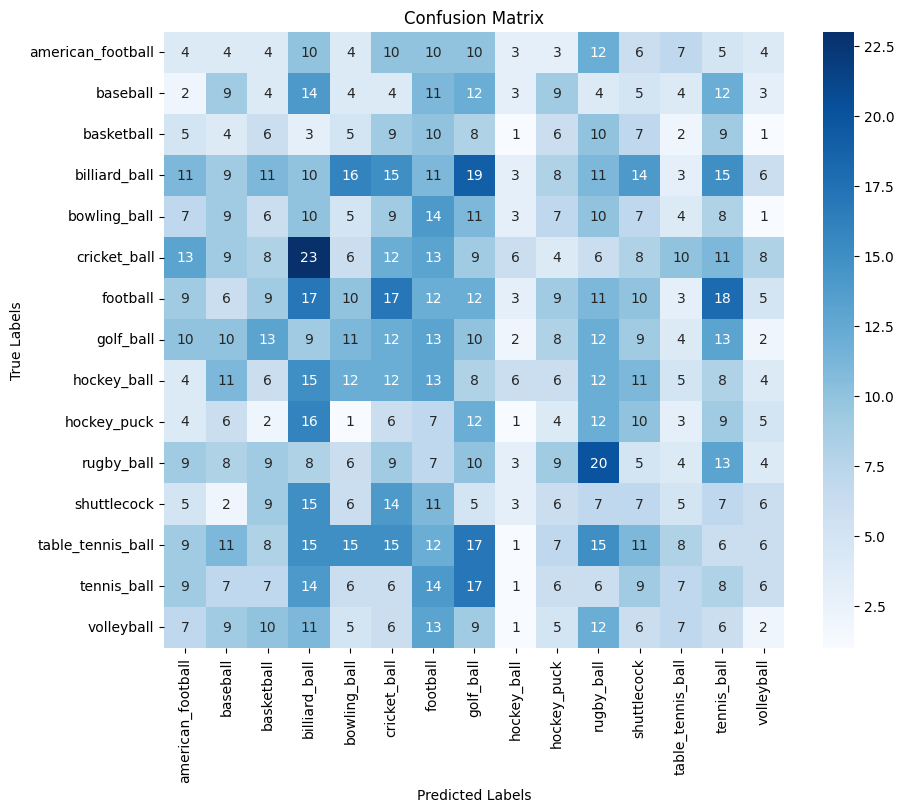
\includegraphics[width=0.7\textwidth]{Labwork6\\download.png}
        \caption{Confusion Matrix}
        \label{fig:confusion_matrix}
    \end{figure}

\section{Conclusion}
Well it works, badly. But it works tho.

For future works, I think we need a dedicatated GPU for each student for training DL model.


\end{document}